\documentclass[10pt]{beamer}

\usetheme{metropolis}
\usepackage{appendixnumberbeamer}

\usepackage{booktabs}
\usepackage[scale=2]{ccicons}
\usepackage{graphicx}
\usepackage{pgfplots}
\usepgfplotslibrary{dateplot}
\usepackage{caption}
\usepackage{subcaption}
\usepackage{xspace}
\newcommand{\themename}{\textbf{\textsc{metropolis}}\xspace}

\title{Bhabha Tracking Efficiencies}
%\subtitle{A modern beamer theme}
\date{01.03.2019}
\author{Martin Sobotzik}
\institute{Johannes Gutenberg Universit\"at Mainz}
% \titlegraphic{\hfill
\includegraphics[height=1.5cm]{logo.pdf}}

\begin{document}

\maketitle
{%
\setbeamertemplate{frame footer}{Bhabha Tracking Efficiencies}

%\section{Reproducing Plots}


\begin{frame}{Motivation}

\begin{itemize}	
	\item I want to study the tracking efficiency of Bhabha processes
	\item For this I first take a look at electrons which are only detected by the ECL
	\item They are therefor labeled and treated as gammas
	\item In the next step I only take information from the ECL and count the electron there without the information from the tracking detectors
	\item Afterwards the number of tracks in the tracking detectors is count to get the efficiency
	

\end{itemize}
\end{frame}
	
\begin{frame}{Getting Started}
	
\begin{itemize} 
	\item Filling the gamma lists:
	
	\begin{itemize}
		\item gamma:probe '$(\textrm{E} > 0.1 )$'
		\item gamma:tag '$(\textrm{clusterE} > 3.0)$'
		\item vpho:cand 'reconstructed from gamma:probe and gamma:tag'
	\end{itemize}

	\item All cuts were taken from Sam's studies:
		\begin{itemize}
			\item $0.296706 < \theta < 2.61799 \rightarrow$ It has to hit the ECL
			\item $\textrm{nCleanedTracks}[ \textrm{abs}(\textrm{dz}) < 2.0 \textrm{ and } \textrm{abs}(\textrm{dr}) < 0.5 \textrm{ and nCDCHits} > 0 \textrm{ and pt } > 0.15] < 1 \rightarrow $ bad quality hits 
			\item $\textrm{M}(\textrm{vpho}) > 8.0\,\textrm{GeV} \rightarrow $ To cut away background (not from his email but surely he is using something like that)					
		\end{itemize}
	
\end{itemize}	
\end{frame}

\begin{frame}{Reproducing Plots}
	
	\begin{itemize}
		\item Sam used Prod6 on all of his plots, and since I try to reproduce his plots I will use it as well
		\item Sam used all Prod6 data. I am only using the following: /hsm/belle2/bdata/Data/release-02-01-00/DB00000438 /prod00000006/e0003/4S/r02*/all/mdst.sub00/*.root
		\item Sam's plots are on the left.	
		\item Three lines. The middle one is $\gamma \gamma$ the two others are $\textrm{ee}$
\end{itemize}
	
	
	\begin{figure}
		\centering
		\begin{subfigure}{.5\textwidth}
			\centering
			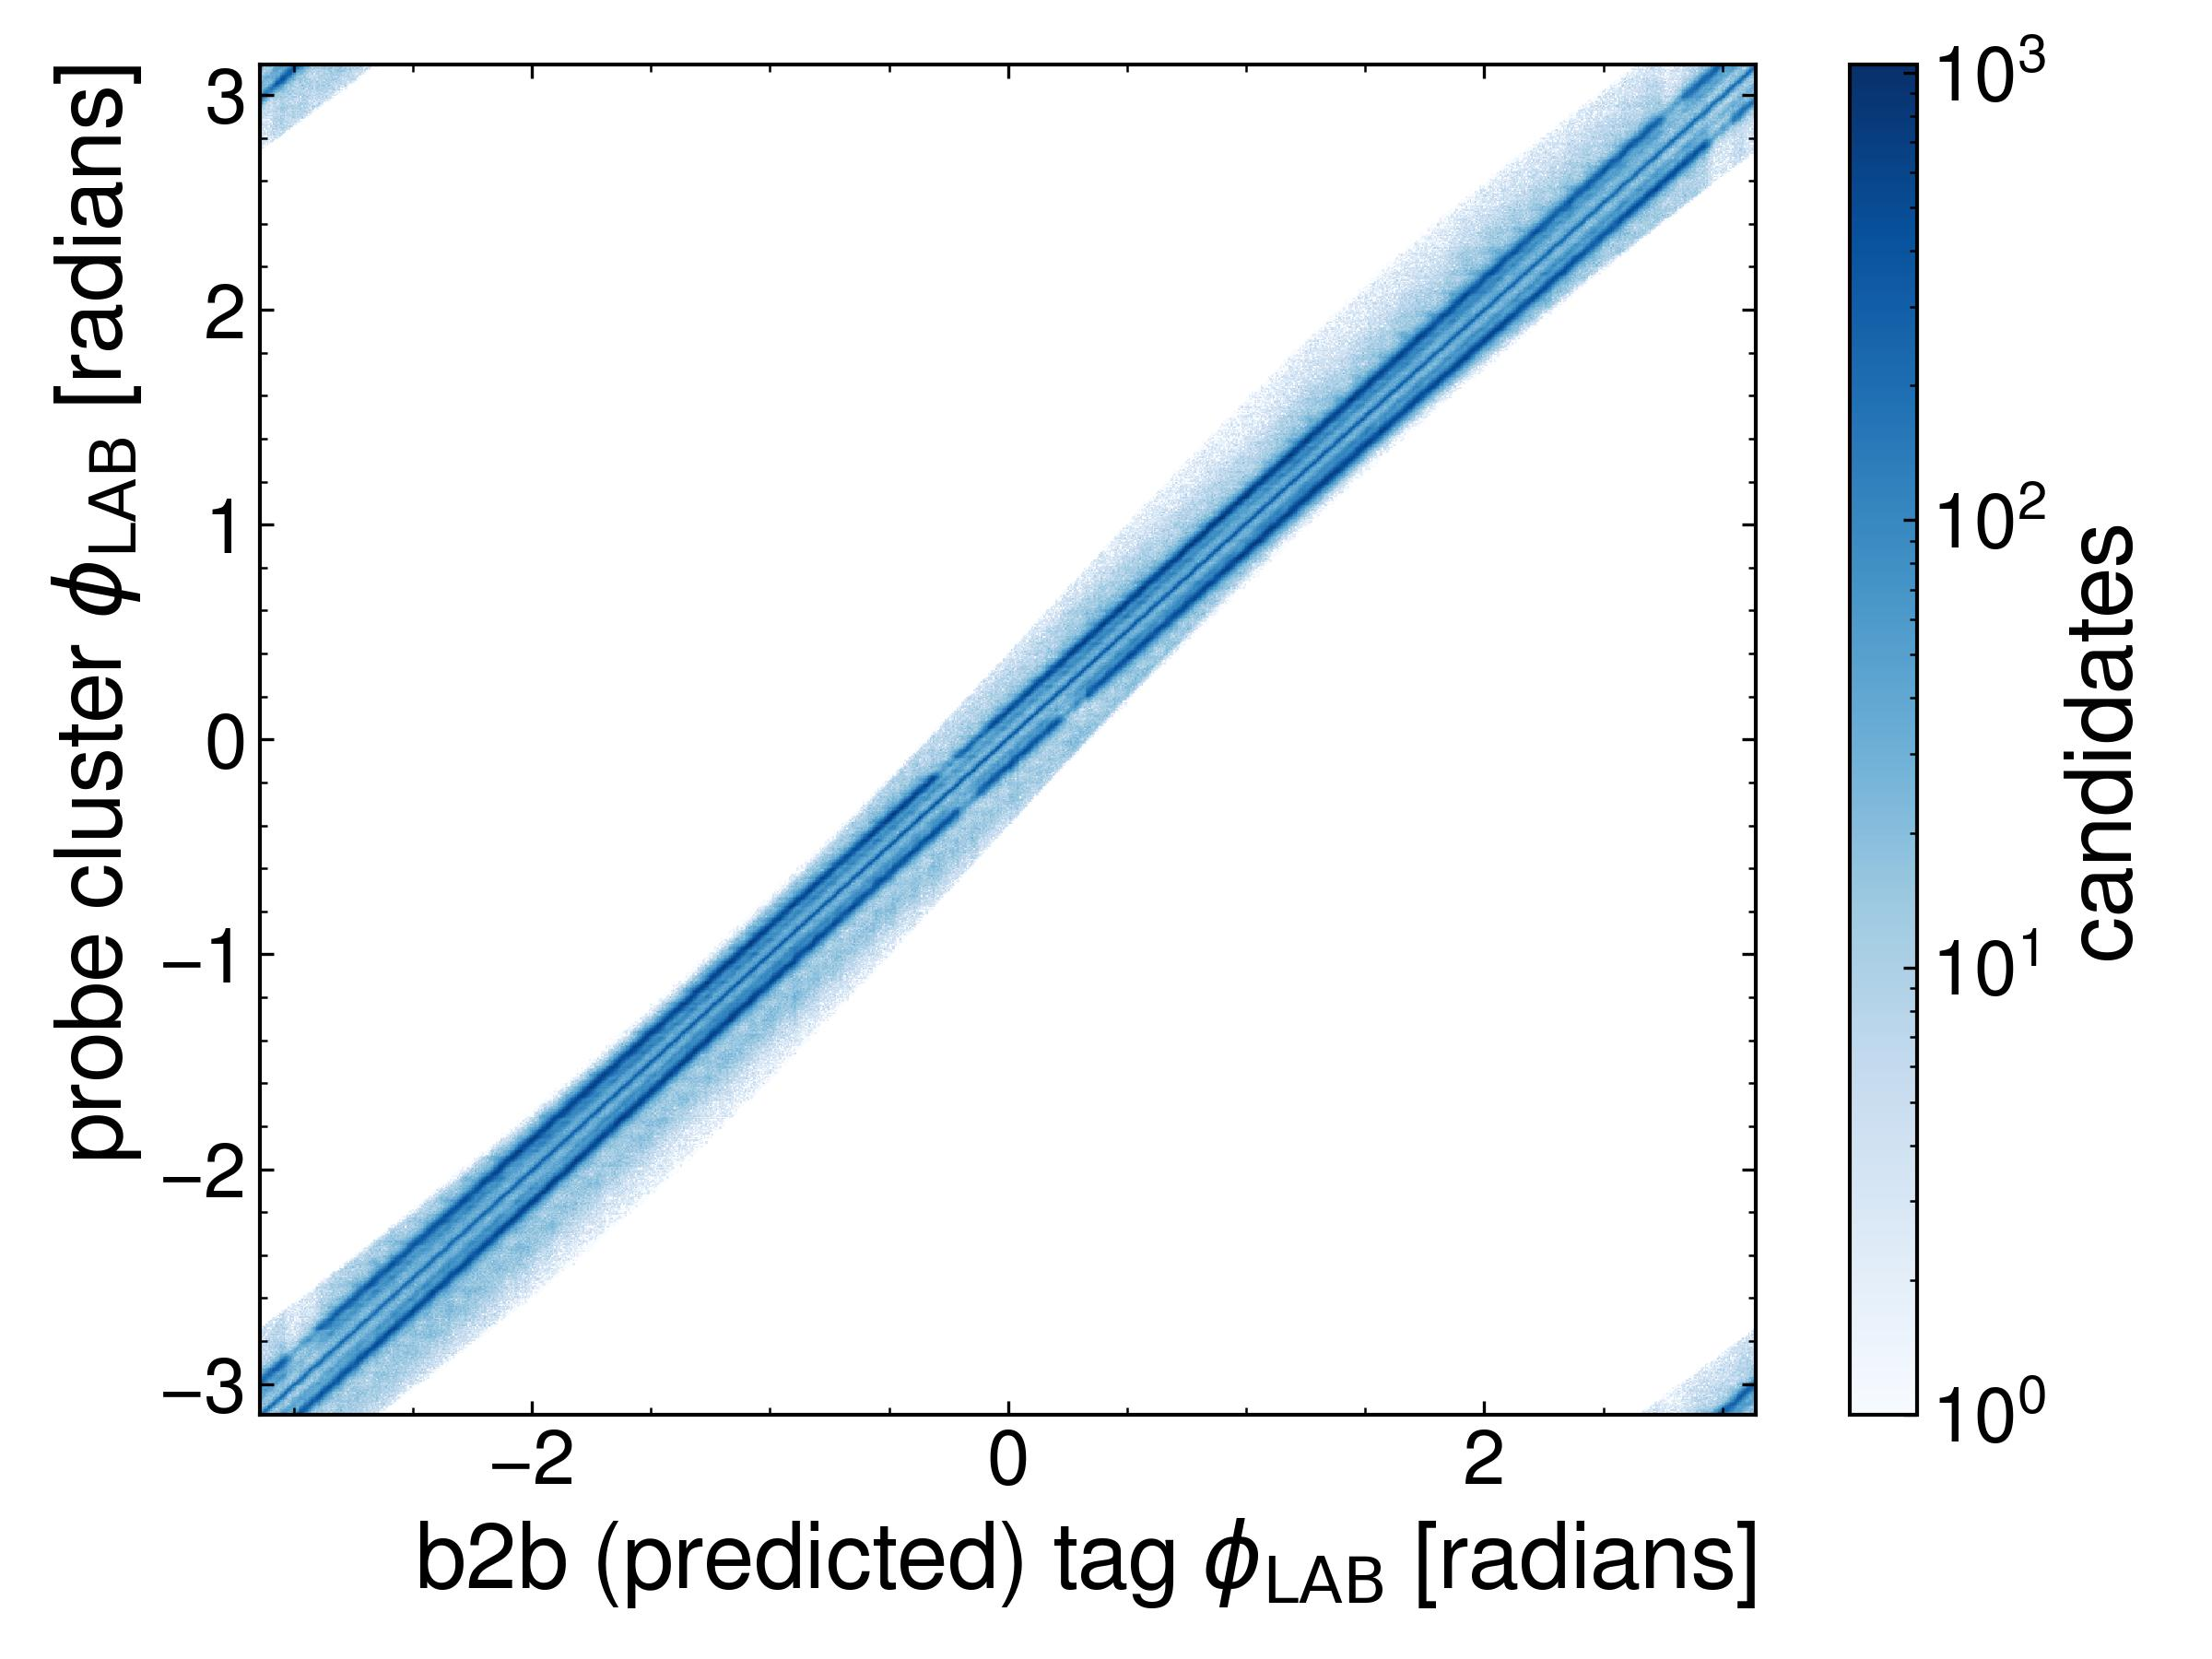
\includegraphics[width=5cm]{Plots/prodRecSam.jpeg}
			
			\label{fig:sub1}
		\end{subfigure}%
		\begin{subfigure}{.5\textwidth}
			\centering
			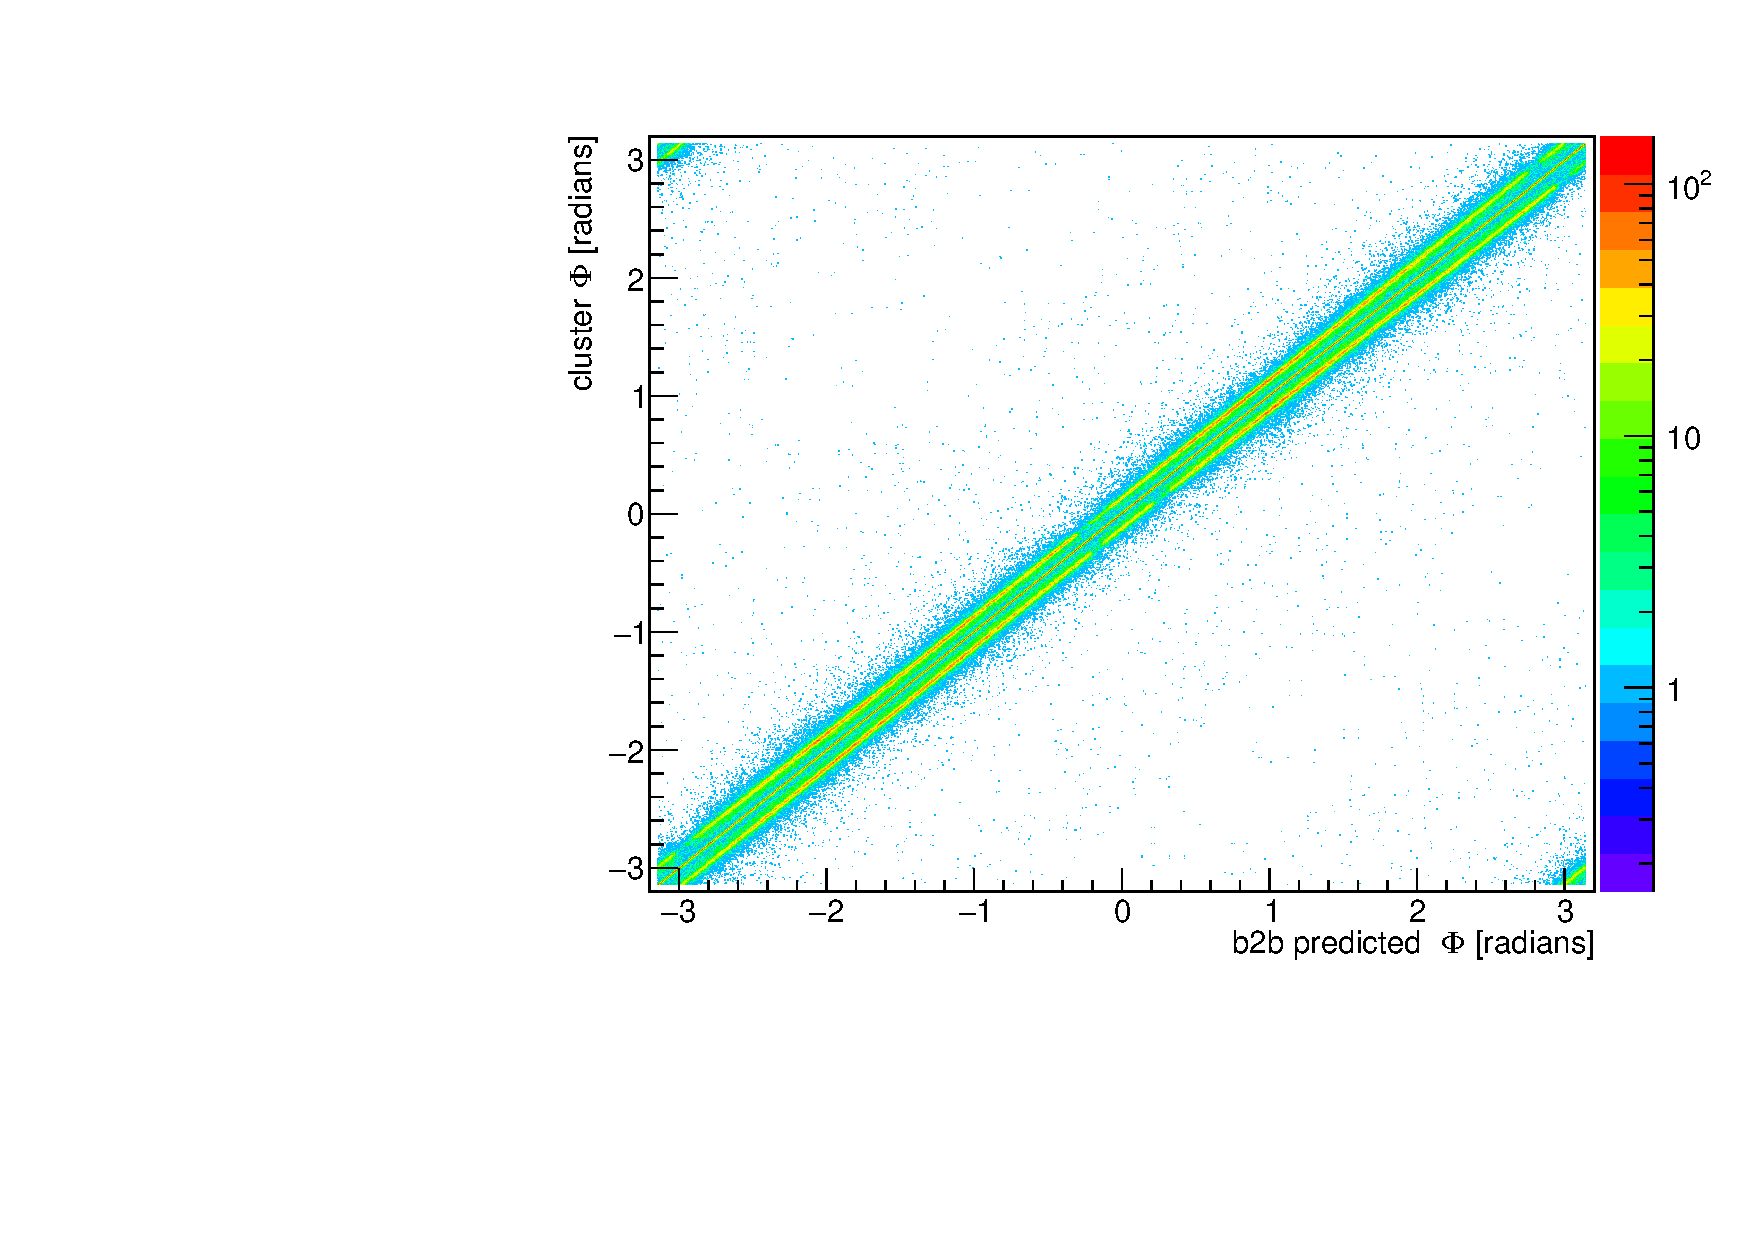
\includegraphics[width=5cm]{Plots/clusterb2b}
			
			\label{fig:sub2}
		\end{subfigure}
				
		\label{fig:test}
	\end{figure}
	
	
\end{frame}


\begin{frame}{Reproducing Plots}
	
	Same plots but zoomed in:
	
		\begin{figure}
		\centering
		\begin{subfigure}{.5\textwidth}
			\centering
			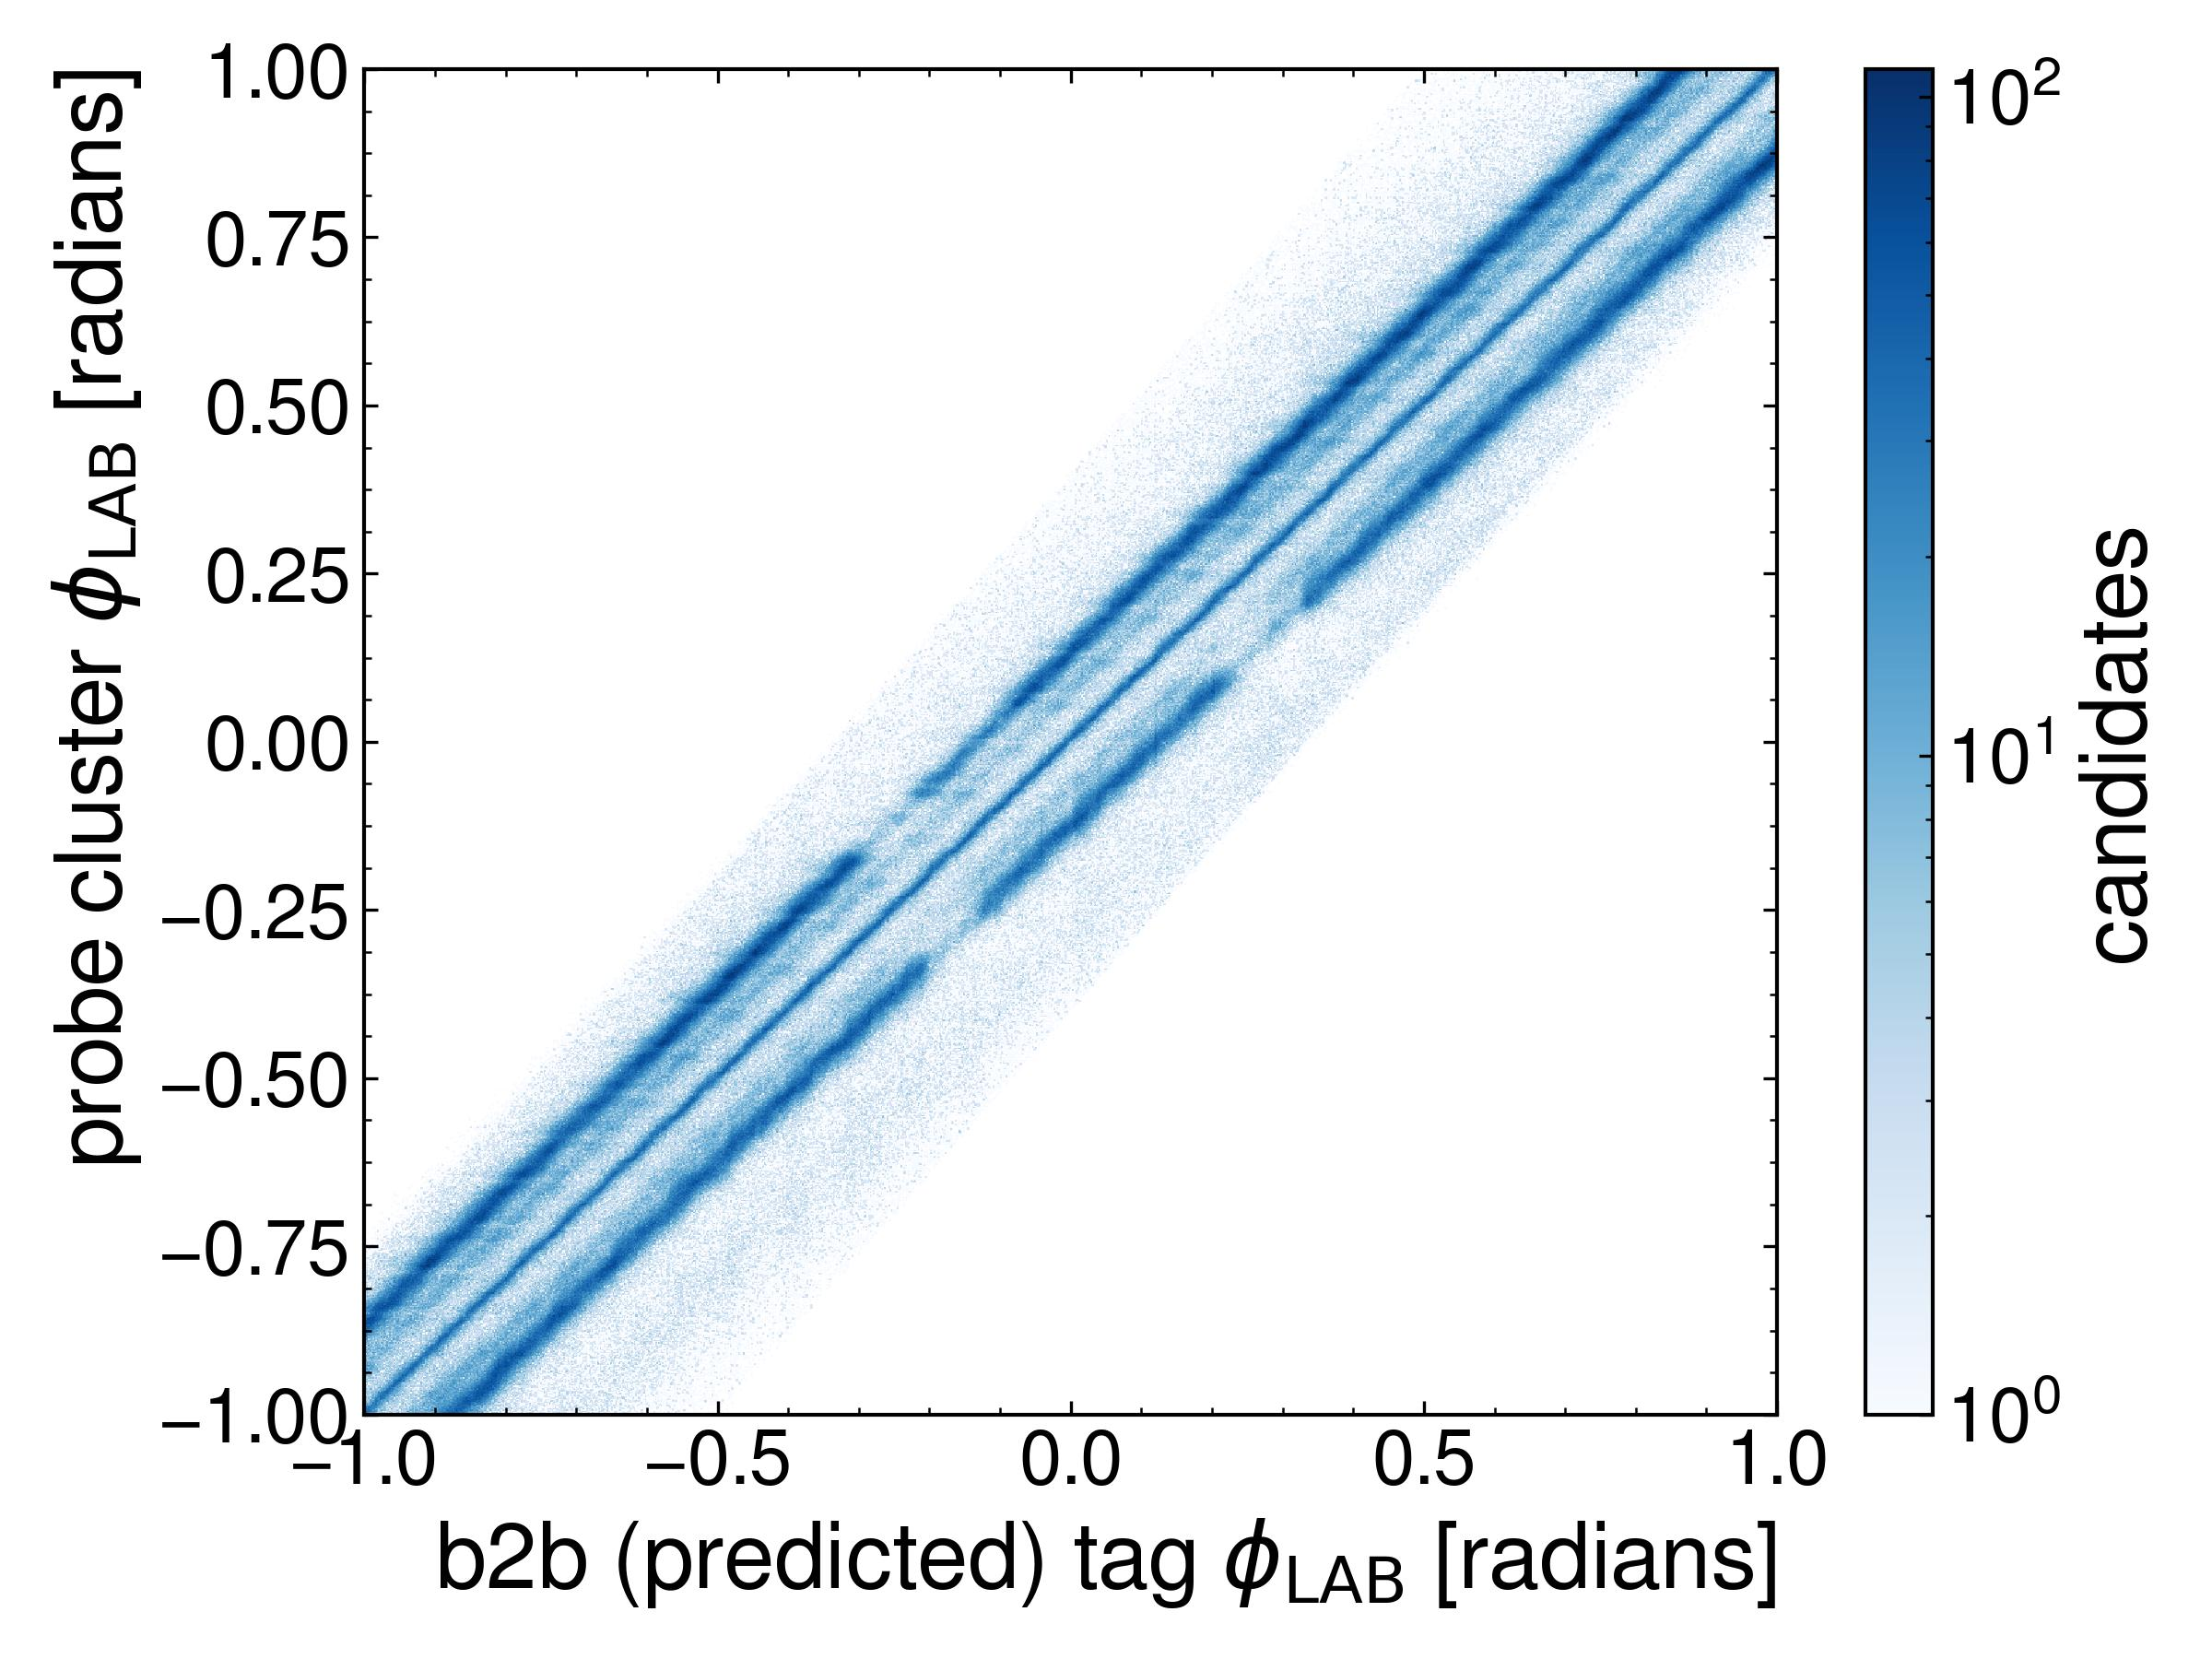
\includegraphics[width=5cm]{Plots/ZommedSam.jpeg}
			
			\label{fig:sub1}
		\end{subfigure}%
		\begin{subfigure}{.5\textwidth}
			\centering
			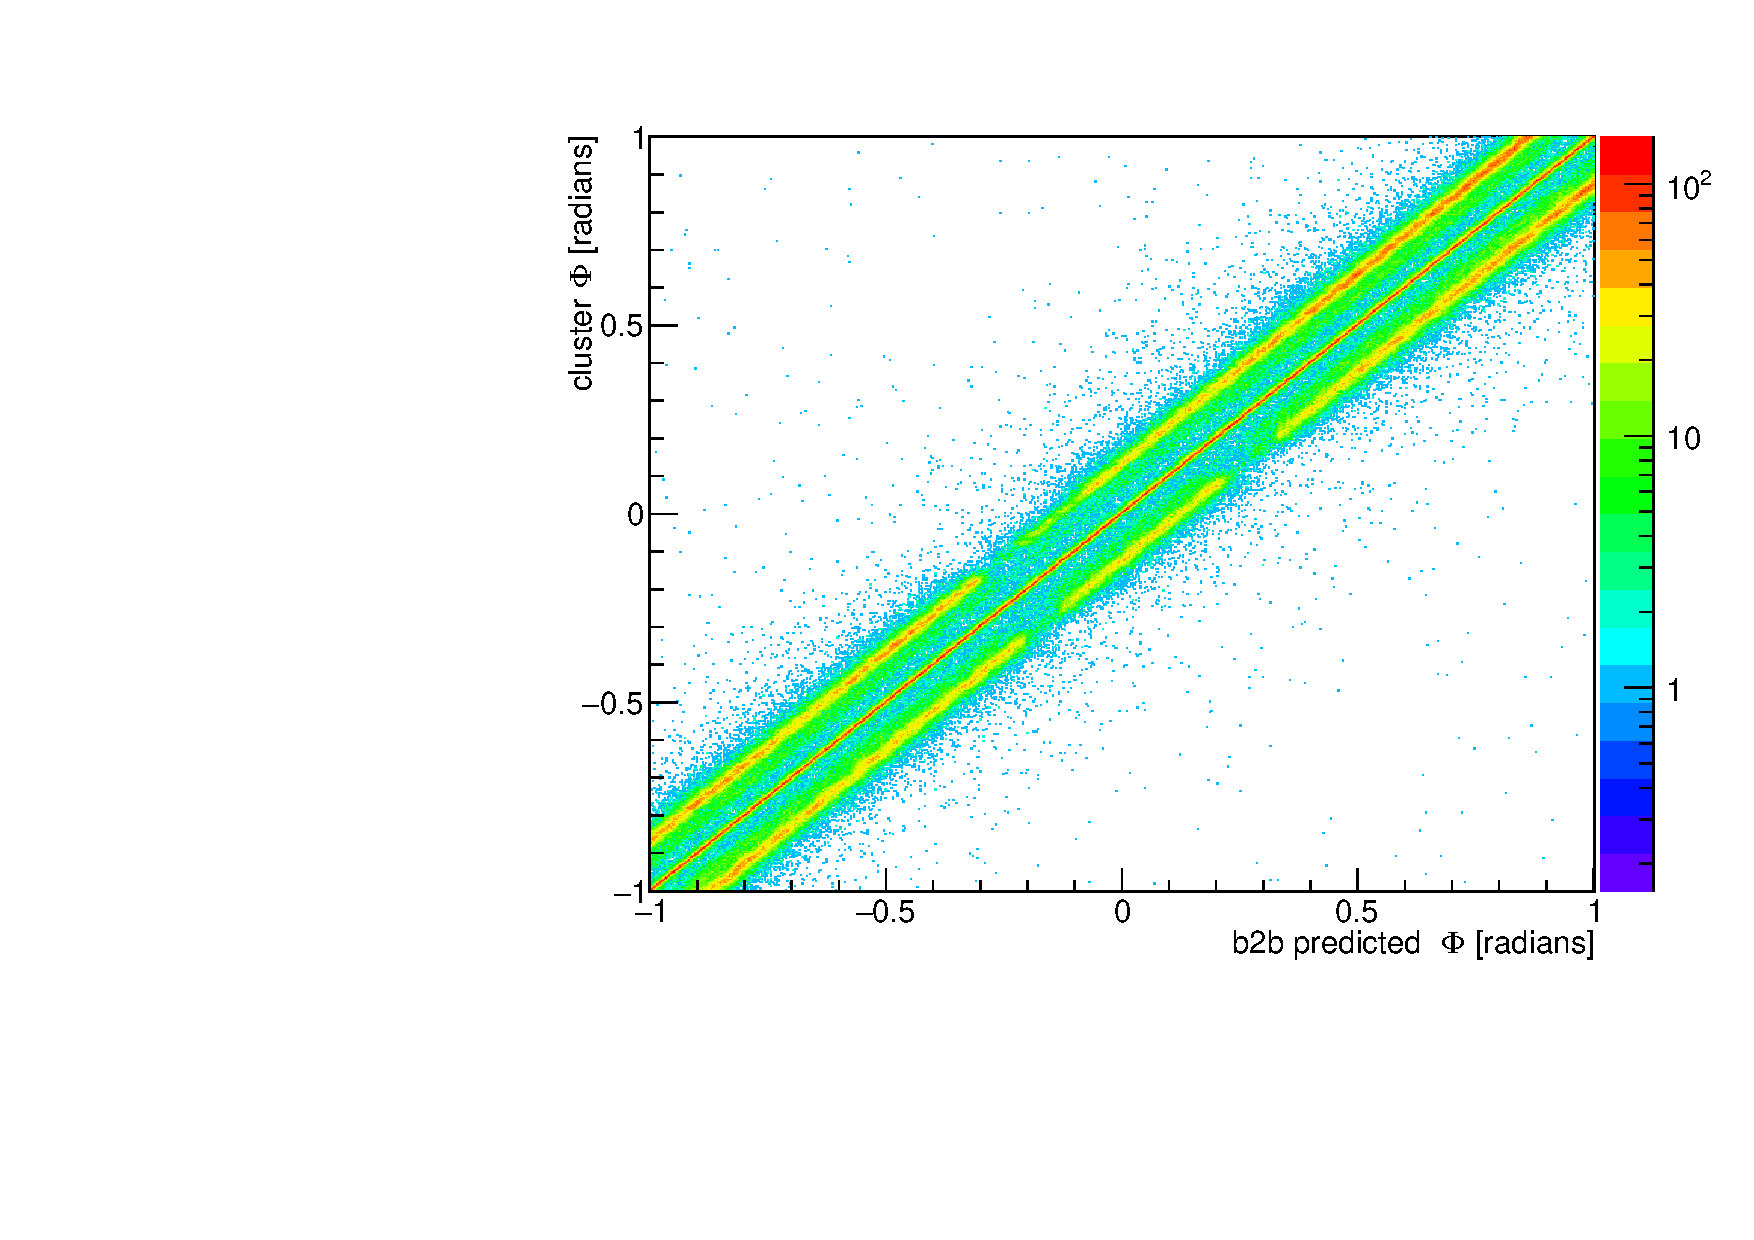
\includegraphics[width=5cm]{Plots/zommedb2b}
			
			\label{fig:sub2}
		\end{subfigure}
		
		\label{fig:test}
	\end{figure}
		
\end{frame}


\begin{frame}{Reproducing Plots}
\begin{itemize} 
	\item The middle peak is $\gamma \gamma$ the two other peaks are $\textrm{ee}$
	\item My $\gamma \gamma$ peak is way higher (Maybe there are some cuts that I am not considering?)

\end{itemize}
\begin{figure}
	\centering
	\begin{subfigure}{.5\textwidth}
		\centering
		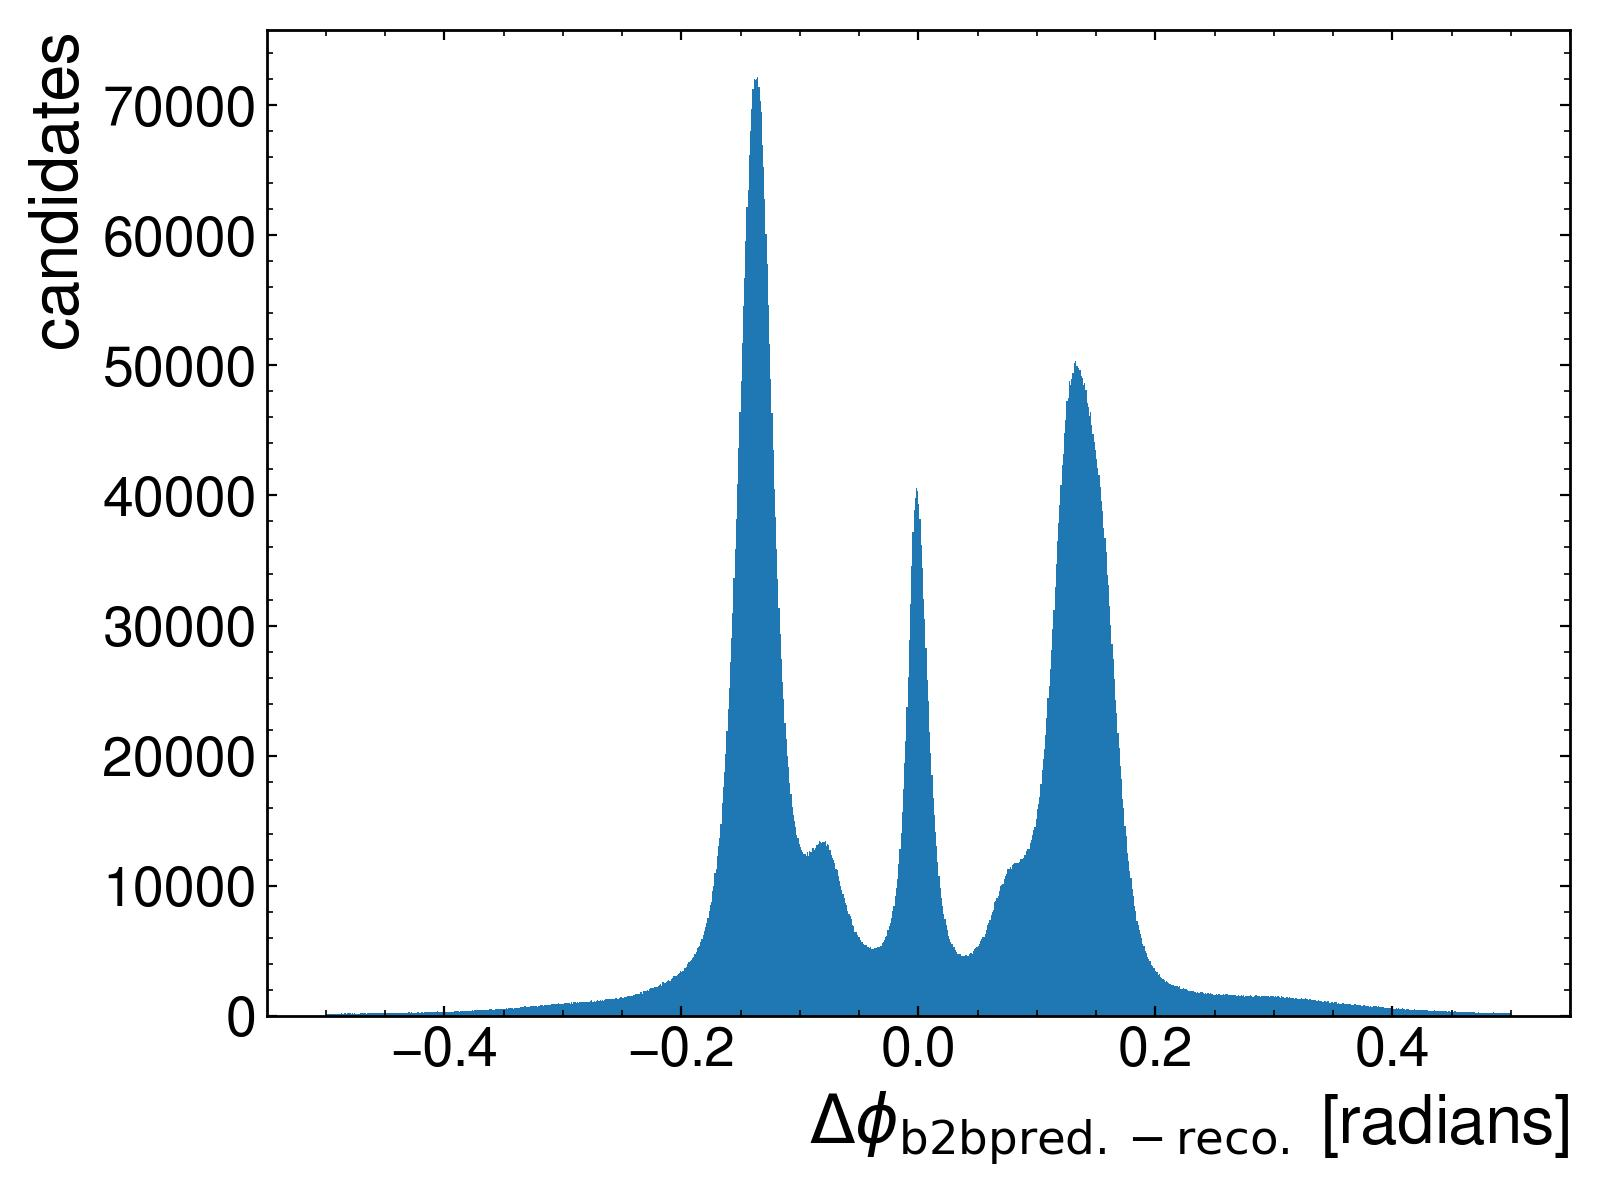
\includegraphics[width=5cm]{Plots/deltaPhiSam.jpeg}
	
		\label{fig:sub1}
	\end{subfigure}%
	\begin{subfigure}{.5\textwidth}
		\centering
		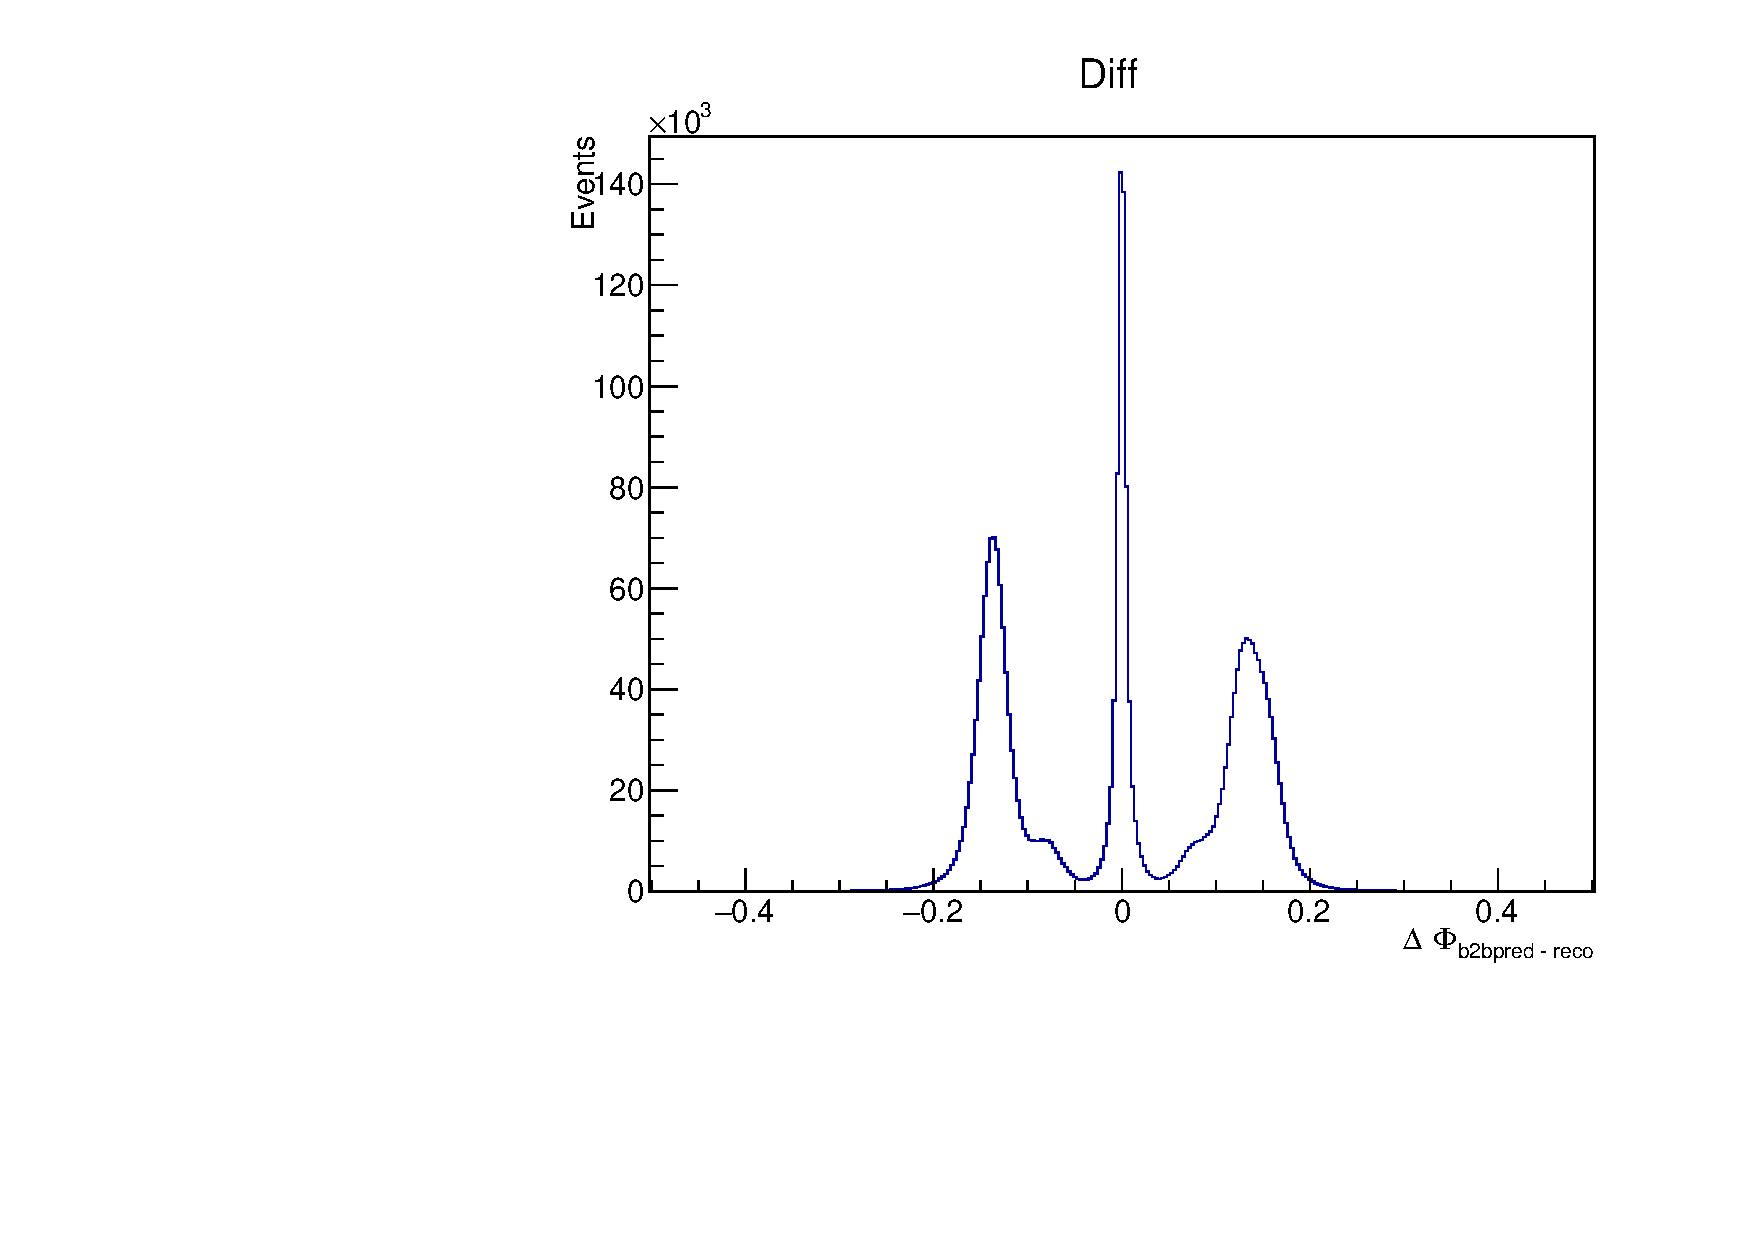
\includegraphics[width=5cm]{Plots/DeltaPhi.pdf}
	
		\label{fig:sub2}
	\end{subfigure}

	\label{fig:test}
\end{figure}

\end{frame}


\begin{frame}{Some more plots}

Here is no Mass cut on the vpho

	
	\begin{figure}
		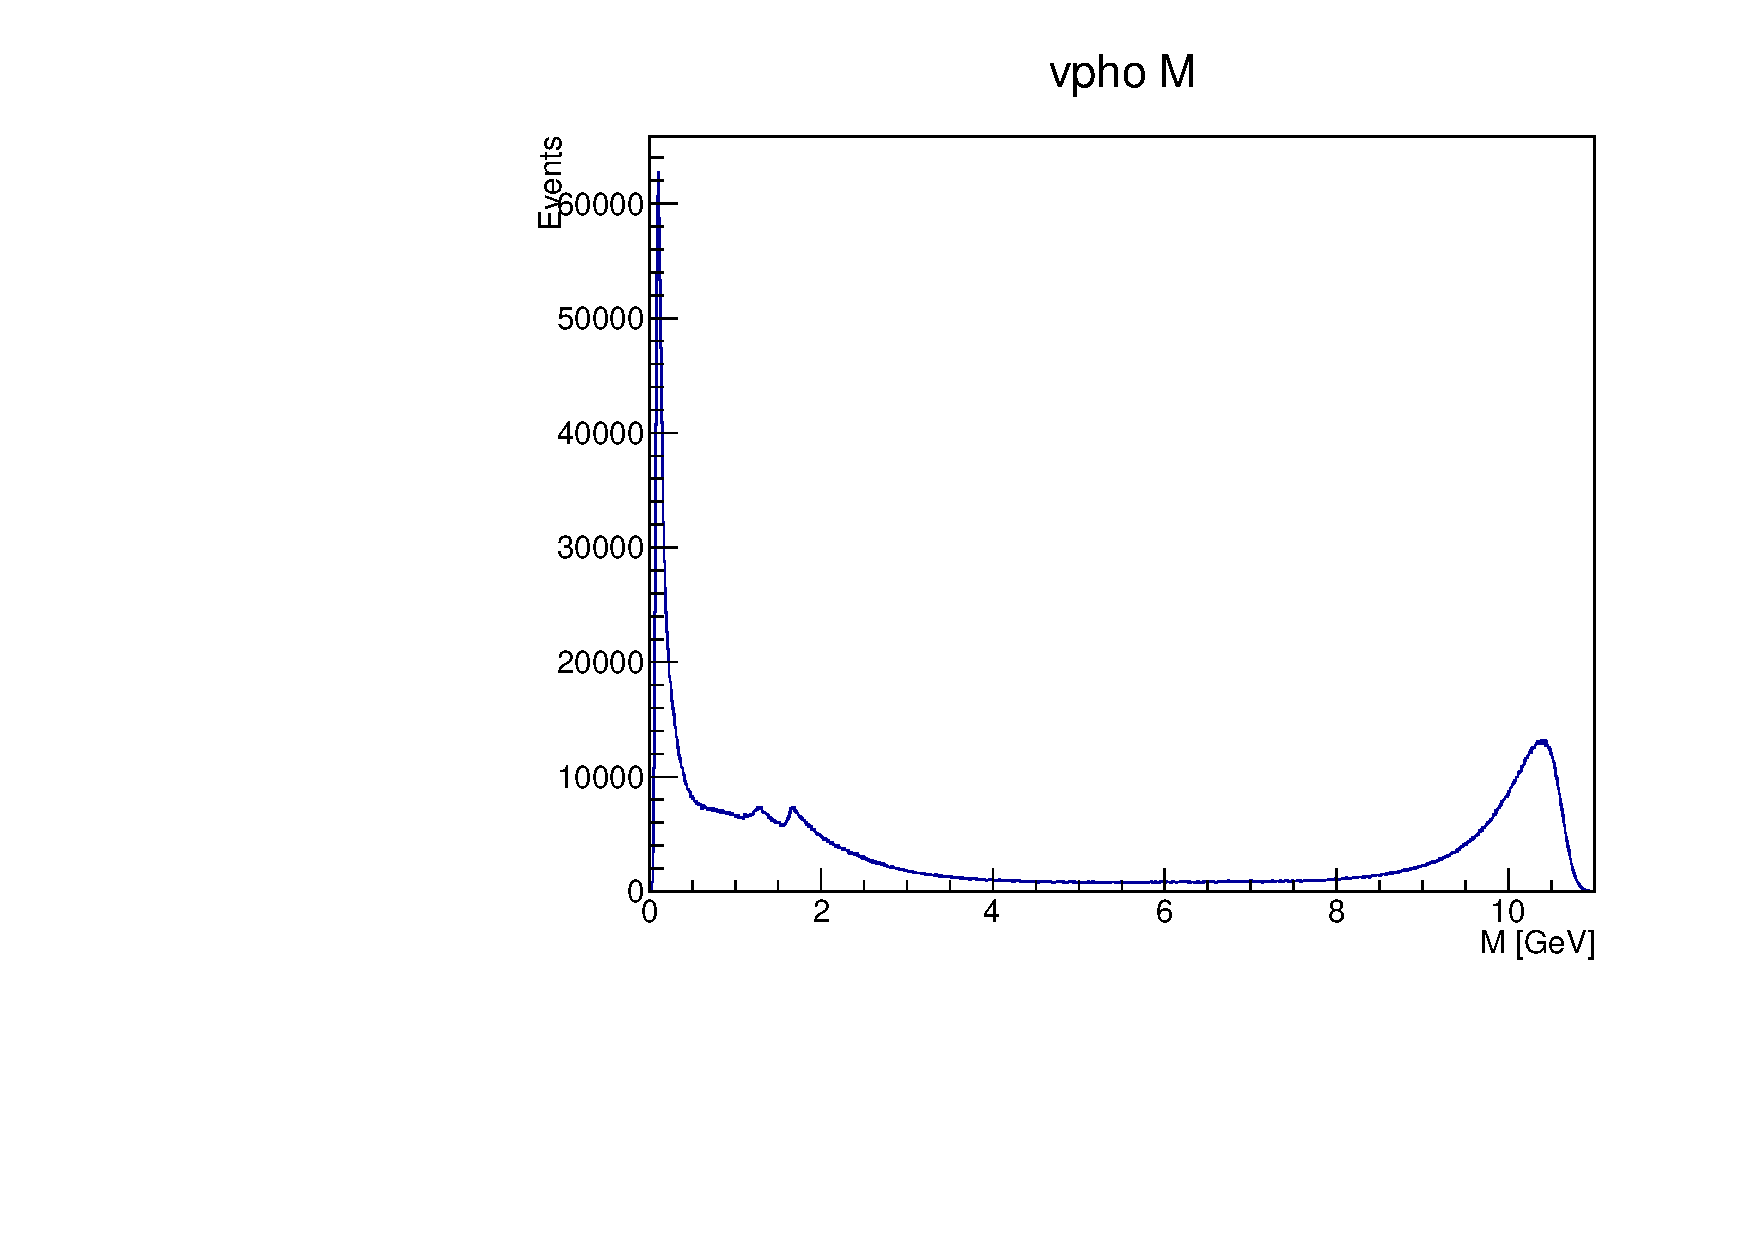
\includegraphics[width=8cm]{Plots/vphoM.pdf}
	\end{figure}
	
	
\end{frame}



\begin{frame}{Some more plots}
	
	\begin{figure}
		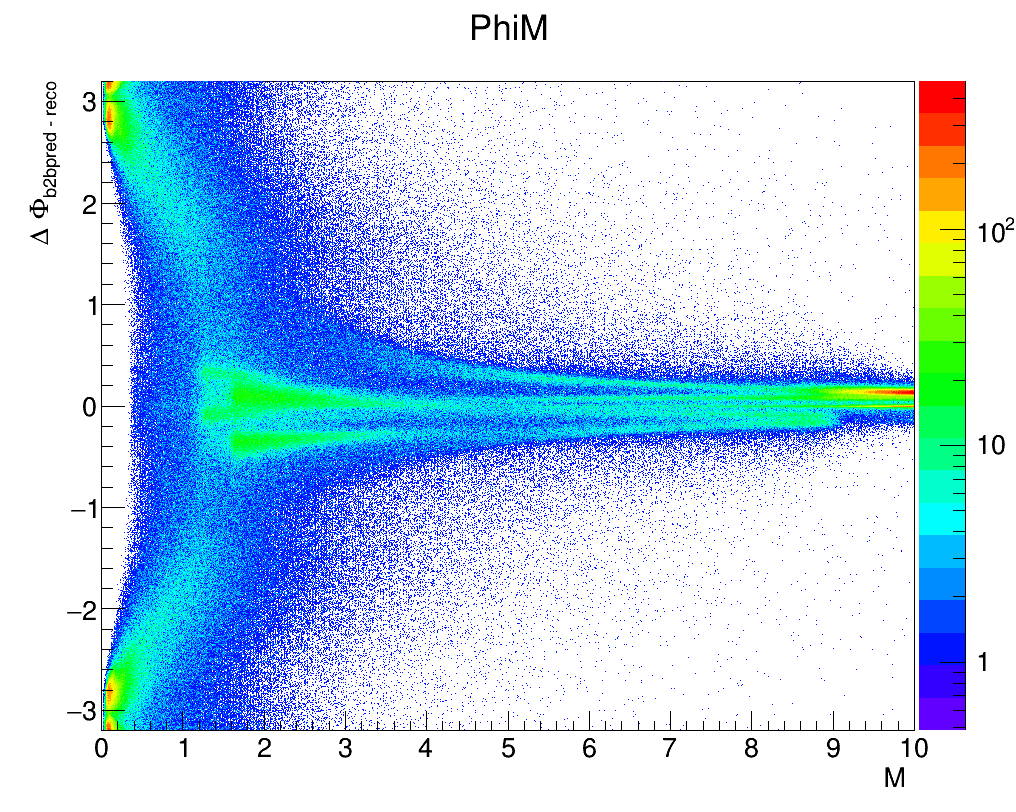
\includegraphics[width=8cm]{Plots/PhiM.png}
	\end{figure}
	
	
\end{frame}

\begin{frame}{Some more plots}
	
	\begin{figure}
		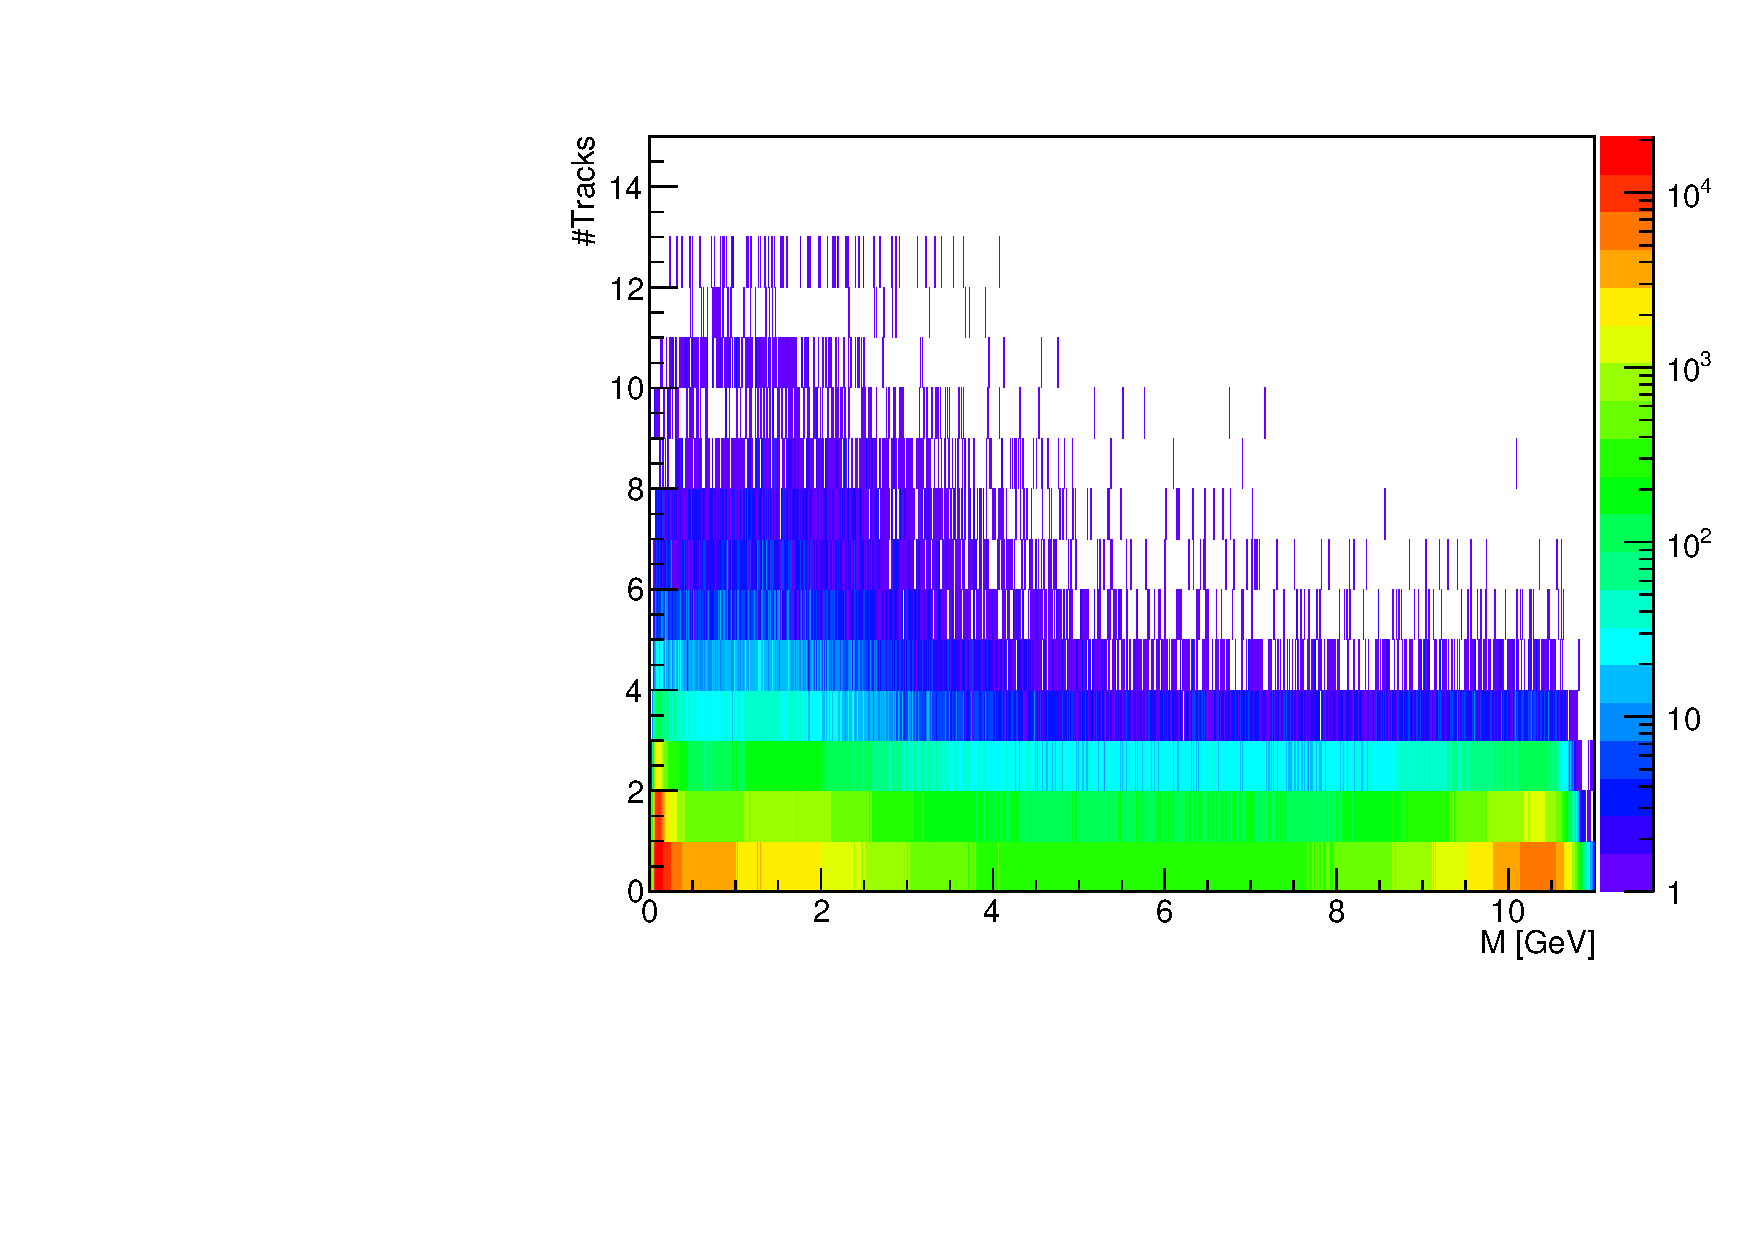
\includegraphics[width=8cm]{Plots/nTrM}
	\end{figure}
	
\end{frame}

\begin{frame}{The next Steps}
	\begin{itemize}
		\item Investigate the best cuts for our purposes and apply them
		\item Select only the $\textrm{ee} $ candidates and study the tracking efficiency using that sample
		\item Producing the same plots shown here using MC sample (from a preliminary study using MC10 it looks like very few events survive applying the descibed selection)
	\end{itemize}
\end{frame}


\end{document}
